\documentclass[10pt]{beamer}
\usepackage[german]{babel}
\usepackage[utf8]{inputenc}
\usepackage{textgreek}
\usepackage{units}

\usepackage[official]{eurosym}


\title[soldering-workshop] % (optional, only for long titles)
{Lötworkshop für Anfänger}
%\subtitle{Löten lernen mit der Maschinendeck Badge}
\usetheme{metropolis}

\begin{document}
    \maketitle
    
    \begin{frame}
    \frametitle{Inhalt}
    \begin{itemize}
    	\item{Was bedeutet Löten?}
    	\item{Benötigte Gegenstände}
    	\item{Wie wird gelötet?}
    	\item{Praxisteil: Löten der Maschinendeck Badge}
    	\item{Links}
    \end{itemize}
	\end{frame}

	\begin{frame}
	\frametitle{Elektroniklöten}
	\begin{figure}[hbtp]
		\centering
		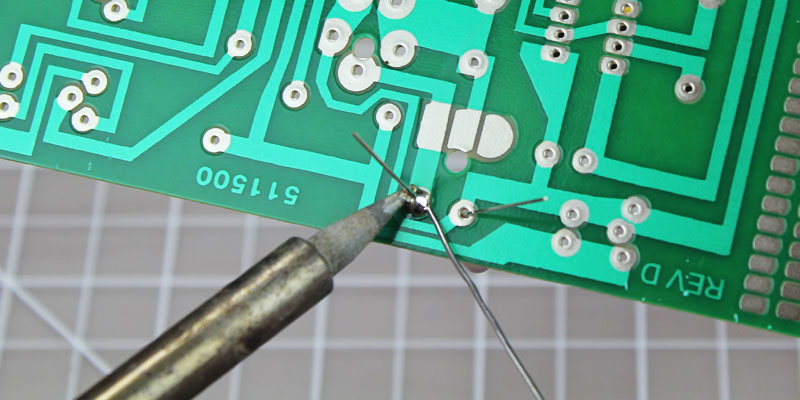
\includegraphics[width=\linewidth*2/3]{images/elektronikloeten.jpg}
		\caption{Quelle: https://www.makerspaces.com/how-to-solder/}
	\end{figure}
	\begin{itemize}
		\item{Verbinden von elektronischen Bauteilen mit einer Platine (PCB)}
		\item{Verwendung von Handlötkolben oder Lötstationen mit \unit[300 - 450]{$^\circ$C} und \unit[30 - 100]{W}}
		\item{Als Metalllegierung wird Lot oder Lötzinn verwendet}
	\end{itemize}
	\end{frame}

	\begin{frame}
		\frametitle{Was wird benötigt?}
		\begin{itemize}
			\item{Bausatz}
			\item{Schutzbrille}
			\item{Lötkolben / Lötstation}
			\item{Lötzinn}
			\item{Seitenschneider}
			\item{Schwamm / Trockenreiniger}
		\end{itemize}
		Optional:
		\begin{itemize}
			\item{Pinzette}
			\item{Dritte Hand}
			\item{Lötdampfabsaugung}
			\item{Lupe}	
		\end{itemize}
	\end{frame}

	\begin{frame}
	\frametitle{Das Lötzinn}
	\begin{itemize}
		\item{Metalllegierung aus Zinn, Blei und anderen Metallen (Elektroniklot)}
		\item{Flußmittelseele zur Verbesserung der Flusseigenschaften im Lot enthalten}
		\item{\textcolor{red}{Beim Erhitzen des Lötzinns können Flussmittelspritzer auftreten. Deshalb nicht zu nahe mit dem Gesicht an die Lötstelle gehen!}}
		\item{\textcolor{red}{Blei ist ein giftiges Schwermetall! Nicht verschlucken!}}
	\end{itemize}
	\begin{figure}[hbtp]
		\centering
		
\includegraphics[width=\linewidth]{images/lotseele.png}
		\caption{Quelle: ERSA Lötfibel}
	\end{figure}
	\end{frame}

	\begin{frame}
	\frametitle{Lötvorgang}
	\begin{figure}[hbtp]
		\centering
		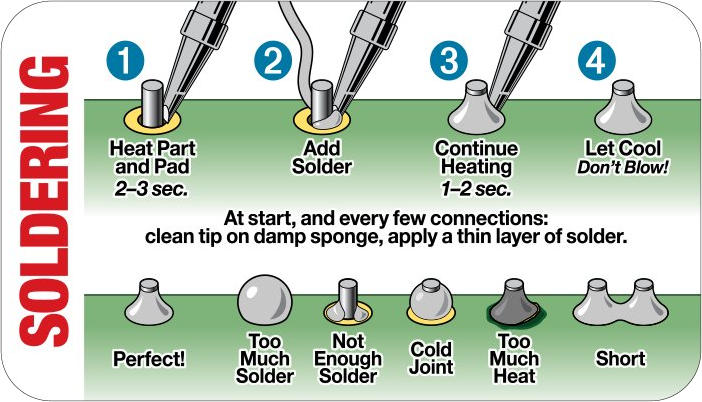
\includegraphics[width=\linewidth]{images/solder.png}
		\caption{Quelle: Adafruit}
		% TODO: Beinchen abschneiden
	\end{figure}
	\end{frame}

	\begin{frame}
		\frametitle{Lötvorgang}
		%TODO: Bilder von lötfehlern einfügen
	\end{frame}

	\begin{frame}
	\frametitle{Praxisteil: Vorbereitung}
	\begin{itemize}
		\item{Arbeitsplatz überprüfen: Lötkolben, Seitenschneider, Lötzinn, Schwamm, Bausatz vorhanden}
		\item{Lötkolben/Lötstation vorgeheizt (\unit[350]{$^\circ$C})}
		\item{Bausatz auspacken und Teile überprüfen}
	\end{itemize}
	\begin{figure}[hbtp]
		\centering
		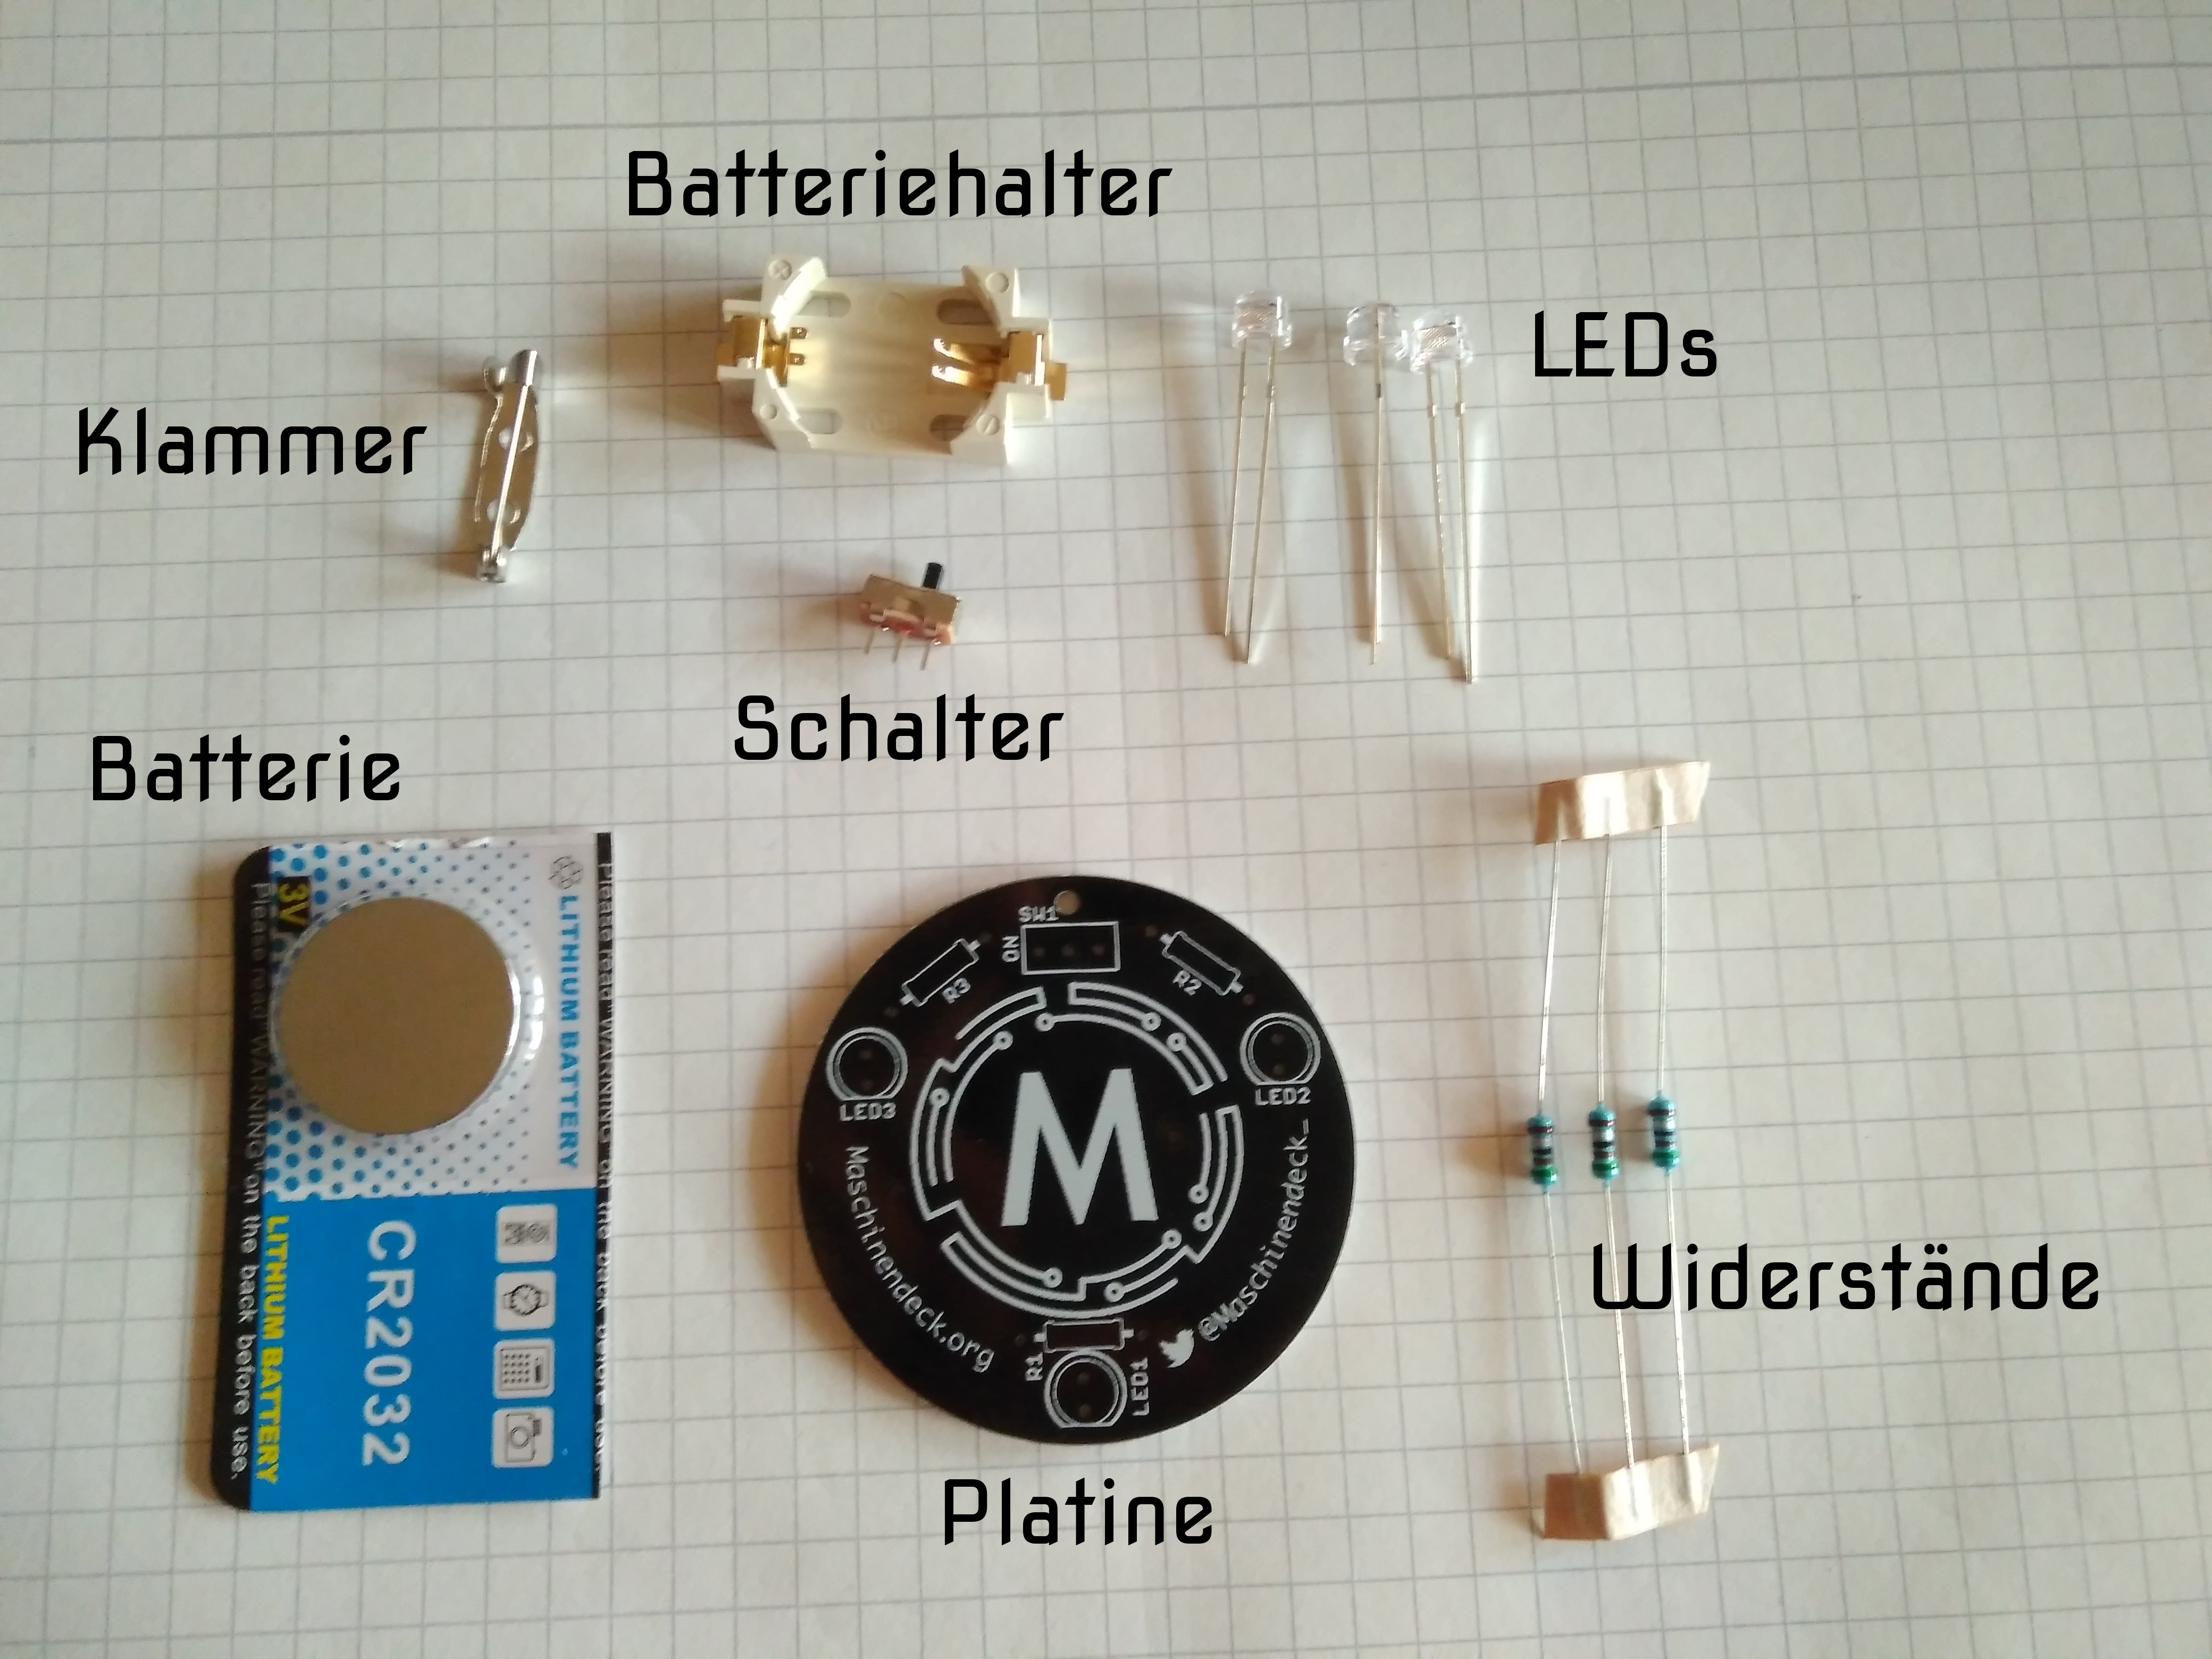
\includegraphics[width=\linewidth*5/10]{images/badge.jpg}
		\caption{Der Bausatz}
	\end{figure}
	\end{frame}

	%\begin{frame}
	%	\frametitle{Praxisteil: Löten der Badge}
	%	 \begin{tabular}{p{\textwidth/3}p{\textwidth/3}p{\textwidth/3}}
	%		\centering 1.
	%		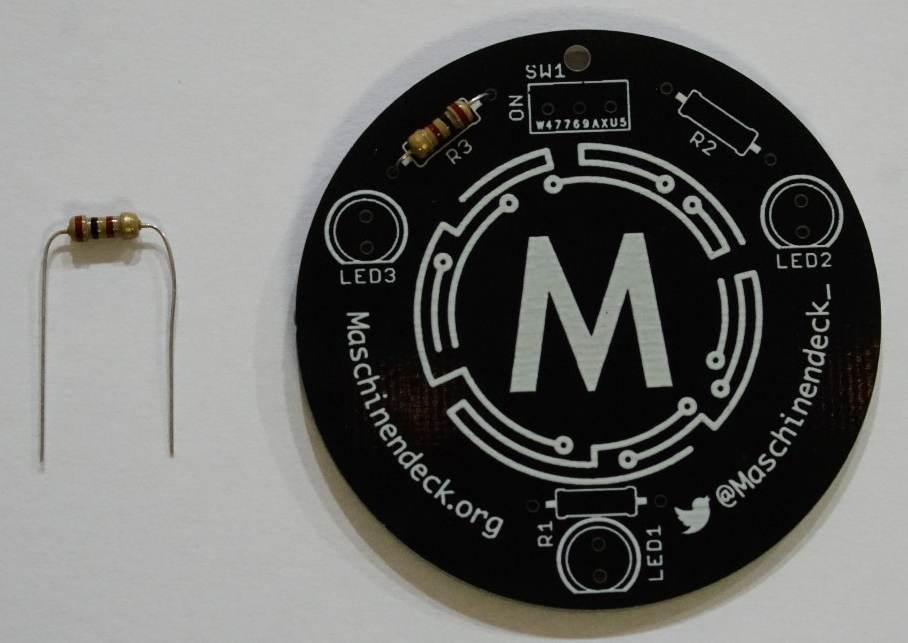
\includegraphics[width=\linewidth]{images/step1.png} & 2. & 3. \\
	%		4. & 5. & 6.
	%	\end{tabular}
	%\end{frame}

	\begin{frame}
		\frametitle{Schritt 1: Löten der Widerstände}
		\centering 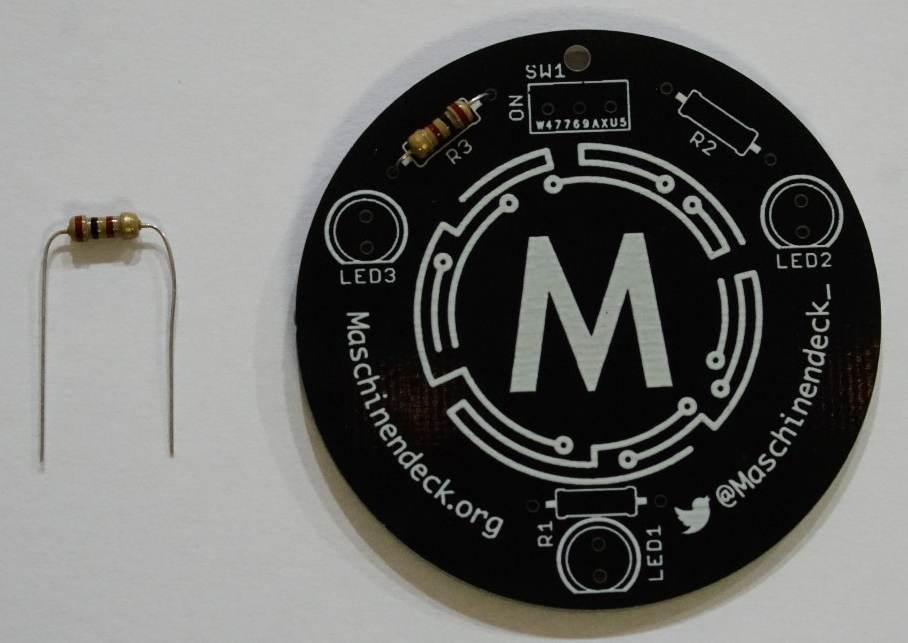
\includegraphics[width=.6\linewidth]{images/step1.png}
		\begin{itemize}
			\item Beinchen der LEDs im richtigen Abstand umbiegen (Biegehilfe)
			\item Durch die Platine stecken und Beinchen auf der Rückseite ein wenig (!) auseinanderbiegen 
			\item Alle LEDs auf der Rückseite verlöten und Beinchen abschneiden			
		\end{itemize}		
	\end{frame}
	
	\begin{frame}
		\frametitle{Schritt 2: Löten der LEDs}
		\centering 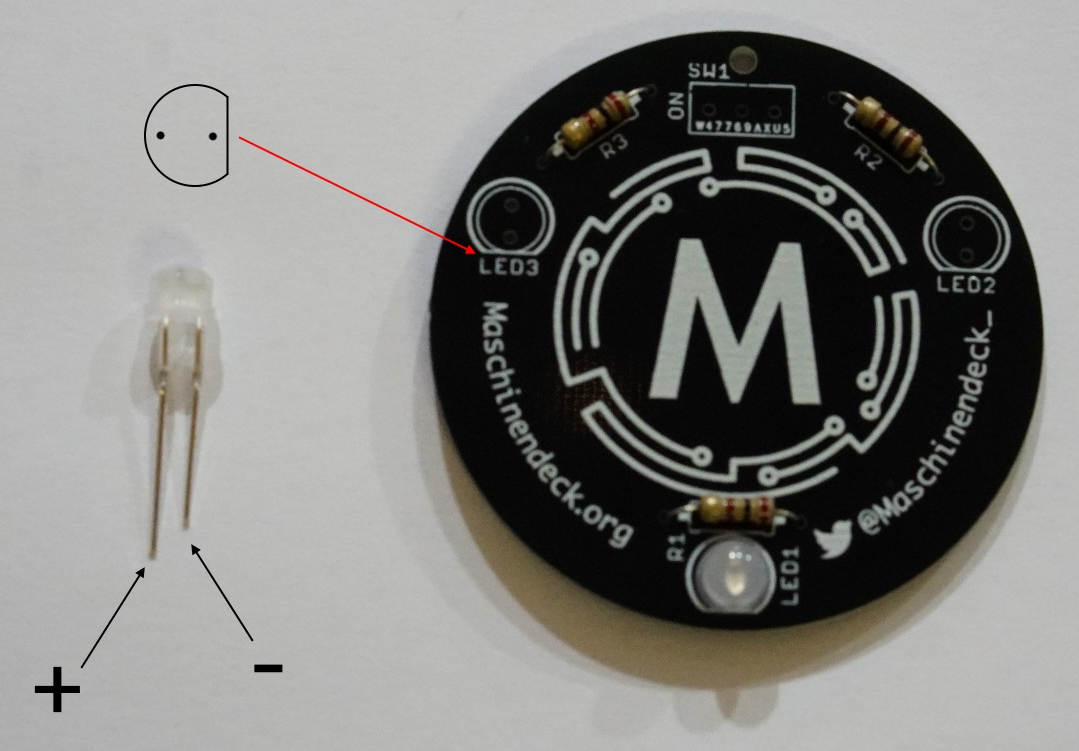
\includegraphics[width=.6\linewidth]{images/step2.png}
		\begin{itemize}
			\item \textbf{Auf richtige Einbaurichtung achten!} Abgeflachte Seite entsprechend dem Symbol auf der Platine
			\item LEDs sind hitzeempfindlicher als Widerstände, deshalb versuchen schnell zu Löten
			\item Alle LEDs auf der Rückseite verlöten und Beinchen abschneiden			
		\end{itemize}
	\end{frame}

	\begin{frame}
		\frametitle{Schritt 3: Löten des Batteriehalters}
		\centering 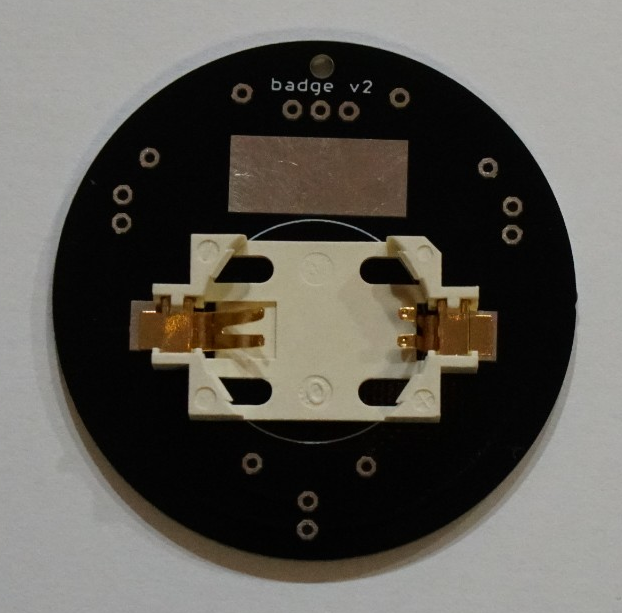
\includegraphics[width=.4\linewidth]{images/step3.png}
		\begin{itemize}
			\item \textbf{Auf richtige Einbaurichtung achten!} Abgeschrägte Seite oben rechts auf der Unterseite
			\item Lötzinn auf Spitze auftragen, Halter mit Pinzette festhalten und zunächst eine Seite festlöten
			\item Danach die andere Seite fest löten und erste Seite evt. nachlöten
		\end{itemize}
	\end{frame}

	\begin{frame}
		\frametitle{Schritt 4: Löten der Anstecknadel}
		%TODO: Bild mit offener anstecknadel + gelöteter batteriehalter
		\centering 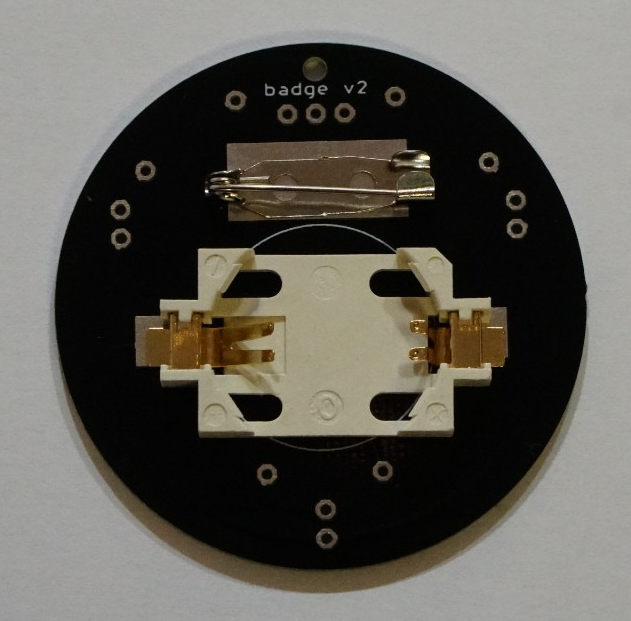
\includegraphics[width=.4\linewidth]{images/step4.png}
		\begin{itemize} 
			\item{Anstecknadel vorher öffnen (vorsicht spitz!) und auf Platine legen}
			\item{Viel Lötzinn und Pinzette zum Festhalten benutzen}
		\end{itemize}
	\end{frame}

	\begin{frame}
		\frametitle{Schritt 5: Löten des Schalters}
		\centering 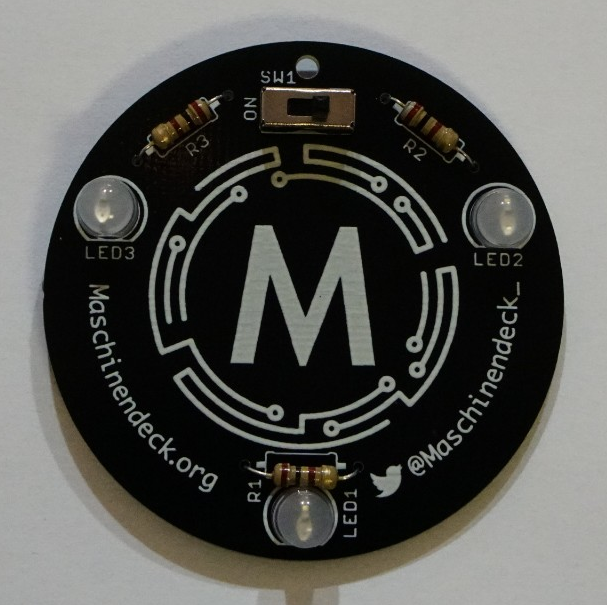
\includegraphics[width=.4\linewidth]{images/step5.png}
		\begin{itemize} 
			\item{Den Schalter von der Vorderseite durch die Platine stecken (Orientierung egal)}
			\item{Zuerst eine Lötstelle löten, dann kann der Schalter noch einmal richtig ausgerichtet werden wenn man diese wieder erhitzt}
		\end{itemize}
	\end{frame}

	\begin{frame}
		\frametitle{Schritt 6: Batterie einlegen und ausprobieren}
		\centering 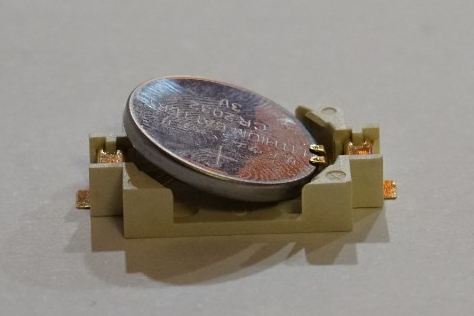
\includegraphics[width=.4\linewidth]{images/step6.png}
		\begin{itemize} 
			\item{Batterie einlegen und den Schalter auf ``ON'' stellen}
			\item{Lötstation ausschalten}
			\item{Lötspitze nicht reinigen, da das verbleibende Lötzinn auf der Spitze eine Schutzschicht bildet}
			\item{Optional: Reinigung der Platine mit Spiritus / Isopropanol / Aceton}
		\end{itemize}
	\end{frame}

	\begin{frame}
		\frametitle{Links}
		%TODO: alignment fixen
		\begin{columns}[] % align columns
			\begin{column}{.5\textwidth}
				\large Präsentation: \normalsize \\
				\vspace{5mm}
				https://github.com/maschinendeck/
				soldering-workshop
			\end{column}
			\begin{column}{.5\textwidth}
				\begin{center}
					
\includegraphics[width=0.6\textwidth]{images/qr-code.png}      
				\end{center}
			\end{column}
		\end{columns}
		
		\large
		Empfohlene Startausrüstung:
		\normalsize
		\begin{itemize}
			%TODO: alles hinter dem doppelpunkt auf einer höhe (tab)
			\item Lötkolben: 	TS100 + Halter + passendes Netzteil
			\item Lötzinn: 		Felder IsoCore Clear Sn96,5Ag3Cu0,5 \textbf{0.5mm}
			\item Schwamm: 		Trockenreiniger aus Messingwolle
			\item Bausätze: 	ELV, Watteroth, Reichelt, Ebay
		\end{itemize}
		
	\end{frame}

	\begin{frame}
	\frametitle{Vielen Dank}
	\centering
	{\LARGE Vielen Dank für eure Aufmerksamkeit!}
	
	\end{frame}
    
\end{document}
